\section{Results}
\label{sec:results}

Tables~\ref{tab:cb} and \ref{tab:main} give every condition and the hypothesis tables every registered test.
Table~\ref{tab:claims} marks each claim below as registered before any confirmatory data (H1--H9), in a later addendum before its
runs (H10--H38), or a re-analysis of data already seen (Appendix~\ref{app:extra});
Table~\ref{tab:evidence} says what each benchmark can support.

\subsection{What a neutral flag does depends on the answer policy}
\label{sec:neutral}
\begin{table*}[t]
\centering\small
\setlength{\tabcolsep}{3.5pt}
\resizebox{\textwidth}{!}{%
\begin{tabular}{lrrrrrrrrrrrr}
\toprule
& \multicolumn{4}{c}{No flags} & \multicolumn{4}{c}{Oracle, neutral flag} & \multicolumn{4}{c}{Oracle, directional flag} \\
\cmidrule(lr){2-5}\cmidrule(lr){6-9}\cmidrule(lr){10-13}
Generator & Correct & Misinfo. & Abstain & Sel. & Correct & Misinfo. & Abstain & Sel. & Correct & Misinfo. & Abstain & Sel. \\
\midrule
\multicolumn{13}{l}{\emph{RAMDocs, multi-answer prompt}} \\
gpt-4o-mini & 22.1 & 47.7 & 3.4 & 22.8 & 15.3 & \textbf{61.9} & 5.0 & 16.2 & 35.5 & \textbf{14.9} & 2.9 & \textbf{36.5} \\
gpt-6-luna & 14.4 & 72.2 & 1.2 & 14.6 & 11.3 & 76.7 & 0.7 & 11.4 & 53.5 & \textbf{11.3} & 1.4 & \textbf{54.3} \\
Claude Haiku 5.5 & 25.2 & 55.2 & 2.2 & 25.7 & 26.4 & \textbf{47.2} & 2.2 & 27.0 & 53.5 & \textbf{6.7} & 2.9 & \textbf{55.1} \\
gpt-6.1-terra & 10.8 & 75.5 & 2.2 & 11.0 & 10.1 & 81.3 & 1.4 & 10.2 & 50.4 & \textbf{13.7} & 2.2 & \textbf{51.5} \\
Claude Sonnet 5.5 & 45.3 & 24.5 & 2.2 & 46.3 & 45.3 & 21.6 & 2.2 & 46.3 & 59.7 & \textbf{3.6} & 1.4 & \textbf{60.6} \\
\midrule
\multicolumn{13}{l}{\emph{ConflictBank, multi-answer prompt}} \\
gpt-4o-mini & 21.6 & 72.8 & 0.3 & 21.6 & 12.8 & \textbf{83.2} & 0.9 & \textbf{12.9} & 49.4 & \textbf{41.2} & 1.2 & \textbf{50.1} \\
gpt-4.1 & 13.0 & 82.7 & 0.7 & 13.1 & 6.7 & \textbf{90.7} & 0.3 & \textbf{6.7} & 36.0 & \textbf{58.3} & 1.0 & \textbf{36.4} \\
Qwen2.5-7B & 23.7 & 67.0 & 6.0 & 25.2 & 15.3 & \textbf{79.0} & 5.0 & \textbf{16.1} & 41.3 & \textbf{52.0} & 13.0 & \textbf{47.5} \\
\midrule
\multicolumn{13}{l}{\emph{ConflictBank, one-answer prompt}} \\
gpt-4o-mini & 51.1 & 31.0 & 6.7 & 54.8 & 32.4 & \textbf{17.7} & \textbf{41.0} & 55.0 & 81.2 & \textbf{4.2} & \textbf{2.1} & \textbf{83.0} \\
gpt-6-luna & 53.6 & 24.3 & 11.9 & 60.8 & 44.1 & \textbf{17.4} & \textbf{28.9} & 62.0 & 90.0 & \textbf{0.0} & \textbf{0.8} & \textbf{90.7} \\
Claude Haiku 5.5 & 66.8 & 22.0 & 1.2 & 67.6 & 67.4 & 22.1 & 0.9 & 68.0 & 90.1 & \textbf{0.2} & 1.1 & \textbf{91.1} \\
gpt-6.1-terra & 73.0 & 18.0 & 1.7 & 74.2 & 70.7 & 15.7 & 4.7 & 74.1 & 90.0 & \textbf{0.7} & 0.3 & \textbf{90.3} \\
Claude Sonnet 5.5 & 75.7 & 15.7 & 1.0 & 76.4 & 78.7 & 12.0 & 1.7 & 80.0 & 92.0 & 1.0 & 1.7 & 93.6 \\
gpt-4.1 & 64.7 & 27.3 & 1.7 & 65.8 & 56.7 & 21.7 & 14.0 & 65.9 & 91.3 & 0.3 & 1.7 & 92.9 \\
Qwen2.5-7B & 50.3 & 35.3 & 5.0 & 53.0 & 47.0 & 28.7 & 15.0 & 55.3 & 75.7 & 13.0 & 1.3 & 76.7 \\
\midrule
\multicolumn{13}{l}{\emph{ConflictBank, forced choice}} \\
gpt-4o-mini & 55.4 & 31.6 & 0.1 & 55.5 & 55.2 & 31.9 & 0.4 & 55.5 & 79.7 & \textbf{6.7} & 0.0 & \textbf{79.7} \\
gpt-6-luna & 64.6 & 25.8 & 0.0 & 64.6 & 66.1 & 22.0 & 0.0 & 66.1 & 91.0 & \textbf{0.1} & 0.0 & \textbf{91.0} \\
Claude Haiku 5.5 & 69.3 & 20.9 & 0.0 & 69.3 & 73.2 & \textbf{16.8} & 0.0 & \textbf{73.2} & 90.4 & \textbf{0.0} & 0.0 & \textbf{90.4} \\
gpt-6.1-terra & 77.7 & 14.7 & 0.0 & 77.7 & 77.3 & 13.3 & 0.0 & 77.3 & 92.3 & \textbf{0.3} & 0.0 & \textbf{92.3} \\
\bottomrule
\end{tabular}}
\caption{Risk and coverage on conflict questions (\%): strictly correct answers, answers that contain the
misinformation, abstentions (``unknown''), and selective accuracy (correct answers over non-abstained answers, pooled
over questions and seeds). \textbf{Bold}: the change from no flags is significant (H21 for
ConflictBank one-answer and forced; the paper's exploratory family elsewhere). The answer policy decides what a neutral
flag does: under a prompt that asks for every valid answer it adds the misinformation to the answer; under a one-answer
prompt that allows ``unknown'' it moves answers, misinformed and correct, into abstention; under forced choice it has
no abstention to trade.}
\label{tab:risk}
\end{table*}


A neutral flag on exactly the gold contradictions lowers gpt-4o-mini's RAMDocs conflict-question accuracy
by \adOracleFlagConf\ points \dOracleFlagConfCI\ from \plainConf\% (H2), and gpt-4.1's by \agptOracleFlagConf\ (H9; Table~\ref{tab:risk} splits it by answer policy).

\paragraph{Asked for every valid answer, the model adds the misinformation.} Under RAMDocs' default prompt,
the flag raises gpt-4o-mini's
misinformation share from \zmRdMiniPlainWrong\% to \zmRdMiniOracleFlagWrong\%: told that two
passages conflict, it reports both sides. Every OpenAI and Qwen generator moves the same way; both Claude models
the other way (Haiku on RAMDocs \zmRdHaikuPlainWrong\% to \zmRdHaikuOracleFlagWrong\%).

\paragraph{Asked for one answer, it abstains.} Under the one-answer prompt, the
flag costs gpt-4o-mini \azSgMiniOracleFlagConflict\ points on ConflictBank, gpt-4.1 \azSgFourOracleFlagConflict\ and
gpt-6-luna \azSgLunaOracleFlagConflict\ (H15, H19), and changes accuracy insignificantly for gpt-6.1-terra,
Qwen2.5-7B, either Claude model (H25) and every generator on RAGuard (H26). Of gpt-4o-mini's misinformed answers, \trSgMiniNeutralMisinfoAbstain\% abstain with the flag, as do
\trSgMiniNeutralCorrectAbstain\% of its correct ones (H21). Under forced choice (H20) its effect is significant only for Claude Haiku
(\hTwentyFcHaikuFlag).

\paragraph{Across settings.} In a multilevel model over the \neuMlK\ settings (Table~\ref{tab:pooled}; exploratory),
fitted with their sampling covariance (shared questions), the pooled effect is \neuMlMu\ points
\neuMlCI\ (\neuMlCIDesign\ conditional on these settings). The effect is
\neuPolMinimal\ \neuPolMinimalCI\ under the minimal prompt, \neuPolMulti\ under
multi-answer, \neuPolSingle\ under one-answer and \neuPolForced\ under forced-choice prompts, and Claude
shifts it up (\neuMlAnthropic; codings chosen after seeing data; utility in Table~\ref{tab:utility}). On WikiContradict, where listing both valid sides is
correct, the flag raises accuracy (H8: \wikiOracleFlag).

\subsection{Naming the false side: what an oracle can deliver}
\label{sec:direction}
With the same oracle pairs, the directional flag beats the neutral and one-wrong flags in every registered comparison
but one (H3, H9--H12, H15, H16, H19, H25, H26; gpt-6.1-terra on RAGuard is not significant). On ConflictBank's
one-answer prompt it gains \azSgTerraOracleFlagDirectionalConflict\ to \azSgLunaOracleFlagDirectionalConflict\
points for the OpenAI generators and \azSgSonnetOracleFlagDirectionalConflict\ to
\azSgHaikuOracleFlagDirectionalConflict\ for Claude. It helps under forced choice (H20) or majority
misinformation, and on RAGuard (H26). On RAMDocs it gains \adOracleDirConf\ points with gpt-4o-mini and
up to \azRdTerraOracleFlagDirectionalConflict\ with gpt-6.1-terra, but not significantly for Qwen2.5-7B or for
gpt-4o-mini under the minimal prompt (H10). On HealthContradict's real web pages it gains \hcDirMini\ to \hcDirHaiku\
points (H37a); the neutral flag, nothing significant (H37b; Table~\ref{tab:hc}). The
one-wrong flag helps only under forced choice (H16, H20).

Oracle rows are a ceiling, not a detector result. An answer key (``the answer $X$ is false'', no passage
marked) does as well: no registered comparison differs significantly (H23; \keyDiffMin\ to \keyDiffMax\ points).
Pooled over the \PoolTwentyThreeK\ comparisons (bootstrapping each benchmark's questions
jointly across them), the flag's advantage is \PoolTwentyThree\ points \PoolTwentyThreeCI, equivalent within $\pm$3 on average
(90\% CI \PoolTwentyThreeCINinety; exploratory). Equivalence rests on the string matcher: an outside-family judge scoring all
\jdN\ responses of the pooled tests puts the flag ahead by \jdTwentyThreeJ\ \jdTwentyThreeJCI, not within $\pm$3
(H38b). Individually, equivalence holds in only \hTwentyThreeEqN\ of
\hTwentyThreeK\ comparisons (between-comparison $\tau$ \hTwentyThreeTau\ points, REML); the arms disagree on \agrTwentyThreeDisMatched\% of question--seed pairs, two no-flag seeds on \agrTwentyThreeNull\%.

\subsection{With a real detector, its wrong flags decide}
\label{sec:real}
\paragraph{Registered results differ by generator.} With the gpt-4o-mini LLM detector, the directional flag significantly raises
accuracy over all ConflictBank questions for \nRealSgPos\ of \nRealSgTests\ generators (gpt-6-luna,
\zSgLunaLlmDirFlagDirectionalLabelled) and significantly lowers it for \nRealSgNeg\ (gpt-6.1-terra,
\zSgTerraLlmDirFlagDirectionalLabelled; H15, H19, H25). It helps all \nRealMjTests\ generators under majority
misinformation, and on RAGuard the two Claude models but no OpenAI one (H26).

\begin{figure}[t]
\centering
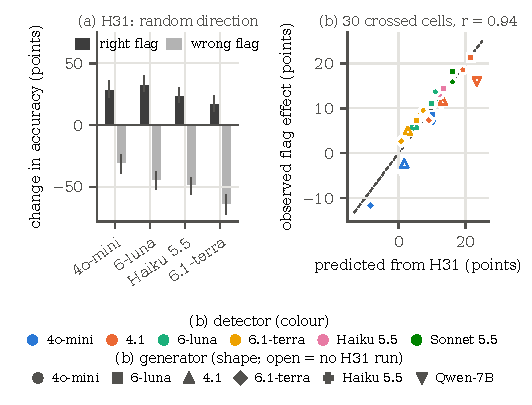
\includegraphics[width=\columnwidth]{generated/fig_reliability.pdf}
\caption{Left: randomised direction (H31; ConflictBank, one-answer prompt): change in accuracy (95\% CIs) on
conflict questions given a right flag (naming the false side) or a wrong flag (naming the correct side). Right: predicted (from H31's follow rates) against observed effect in the \predAllN\ crossed detector--generator
cells (filled: the generator's own rates; open: mean rates, for generators
with no H31 run); dashed: $y=x$. Exploratory and retrospective: the account was defined after the cells
(Table~\ref{tab:cells}) were seen.}
\label{fig:reliability}
\end{figure}
\paragraph{A wrong flag costs more than a right one gains.} In a randomised test (H31), each ConflictBank conflict
question was flagged on its true contradiction, naming the false side for a random \nRandRight\ and the
correct side for the other \nRandWrong. A right flag raises accuracy by \hThirtyOneAMin\ to \hThirtyOneAMax\ points and
a wrong one lowers it by \ahThirtyOneBMax\ to \ahThirtyOneBMin\ (Figure~\ref{fig:reliability}, left). The net effect is
significantly negative for \nHThirtyOneCSig\ of \nHThirtyOneCTests\ generators at an even mix (H31c).
For right- and wrong-flag effects $R$ and $W$, randomised flags on true pairs do net harm below a break-even
direction precision $p^\star=-W/(R-W)$: \beMini\ \beMiniCI\ for gpt-4o-mini, \beLuna\ for gpt-6-luna, \beHaiku\ for Claude
Haiku and \beTerra\ \beTerraCI\ for gpt-6.1-terra (Table~\ref{tab:breakeven}; exploratory). Follow rates overlap except gpt-6.1-terra's,
so $p^\star$ rises mainly because an accurate generator has more to lose. The threshold is a calibration, valid for a real
detector only if it flags typical questions and nothing else.

\paragraph{Real detectors are selective.} Across H24's \hTwentyFourCells\ cells
(Table~\ref{tab:selection}), comparing precision with $p^\star$ can mislead. The gpt-4o-mini detector's precision
(\selHaikuMiniPrec\%) is just above Claude Haiku's break-even, implying \selHaikuMiniMarg\ points, but the cell's effect is
\selHaikuMiniObs: its flags on a correct passage (\selHaikuMiniWrongShare\% of questions) change accuracy there by
\selHaikuMiniWrongGain. The follow-rate account
$\hat\Delta=\frac1n\sum_i[d_i(1-a_i)f_R-w_ia_if_W]$ ($d_i$: the flag names the false side; $w_i$: it marks a correct
passage; $a_i$: no-flag accuracy; $f_R,f_W$: H31's follow rates), defined after the cells were seen, tracks the
\predEightN\ cells with an H31 generator (mean error \predEightMae\ points; Figure~\ref{fig:reliability}).
The registered H24 correlation is uninformative, since generator accuracy enters both sides. The least precise detector (gpt-4o-mini, \dirPrecMini\%) lowers accuracy for the four most
accurate generators, significantly for gpt-6.1-terra (H19).

\paragraph{Frozen in advance, the account predicts new cells (H32).} On 400 unseen ConflictBank questions, five
detectors (one new) crossed four generators; predictions from detections and no-flag answers were committed before
any flagged answer existed. Over the \frN\ cells the slope is \frSlope\ \frSlopeCI\ and the mean error \frMae\
points, against \frMaeGen\ for generator means (cell-level rates alone: \frMaeMarg). The sign is right in all
\frBigN\ cells predicted at $\ge$3 points, but only \frHarmConf\ of \frHarmN\ predicted harms is significant (H33 fails). The account overstates harm on clean questions (\frCleanPred\ vs \frCleanObs) and
on HealthContradict (gpt-6-luna \hcLlmPredLuna\ vs \hcLlmLuna; Table~\ref{tab:fresh}, Appendix~\ref{app:fresh}).

\paragraph{In mean accuracy, the detector's verdict carries most of its contribution.} The detector's judgement, passed as an answer key,
matches the directional flag (H30, no cell significant): pooled over the \PoolThirtyAK\ cells the flag
is ahead by \PoolThirtyA\ \PoolThirtyACI, equivalent within $\pm$3 under the matcher; under the judge,
\jdThirtyJ\ \jdThirtyJCI\ (not within $\pm$3, H38a). The key says ``the
answer $X$ is false'' for the answer the benchmark labels its suspect passage as supporting: an information-content
control, not a deployable format. The flag beats the detector model's own-answer
hint by \PoolThirtyB\ \PoolThirtyBCI\ (H27).

\paragraph{With rare conflicts, false flags can outweigh gains.} The LLM detector also flags clean questions
(\cleanFprLlm\% of RAMDocs'). At a 5\% share of conflict questions its flag's estimate is negative in \prevNegFive\ of \prevN\ correlated settings
(significantly in \prevSigNeg; Table~\ref{tab:prevalence}).

\paragraph{Genuine conflicts and baselines.} Reordering \citep{liu2024lost} or paraphrasing passages does not significantly
change the detectors' hit rate (H29). Where both sides are valid, direction does damage (H28): on WikiContradict the LLM directional
flag lowers the share of answers giving both sides by \ahTwentyEightWcMiniDir\ to \ahTwentyEightWcLunaDir\ points
(and of answers correct under the benchmark's own rubric by \awikiOrigMiniEffPt\ to \awikiOrigLunaEffPt;
Appendix~\ref{app:semantic}). On RAMDocs' same-name questions, removal costs every generator
\ahTwentyEightAmbMiniRem\ to \ahTwentyEightAmbLunaRem\ points. Baselines: Appendix~\ref{app:extra}.
